% !TeX root = ./00.ppgcc-2020.tex

\chapter{Trabalhos Relacionados}\label{cha:related}

% \notaPA{Sugestão na Estrutura:
% Eu deixaria como Cap 02 ou como Cap 05.
% Acho que um Cap de Trabs Relacionados no meio da dissertação quebra o fluxo de leitura.}
% Author: Lets try this

% % discussão de 2020-02-01
% Aqueles que contenham:
%     - detecção de anomalia em streams
%     - detecção de intrusão em rede com processamento de streams
%     - BigFlow
% %/discussão

% cap 3: Trabalhos relacionados
%     - Artigos sobre o Minas
%     - outros que paralelizaram algoritmos de mineração de 
%        dados/streams alguns online (5-10 refs)
%     - implementação paralelas/distribuídas em dispositivos pequenos
% % 

Este Capítulo trata dos trabalhos relacionados e apresenta aspectos do estado da
arte dos tópicos Detecção de Novidades em Fluxos de Dados e Processamento
Distribuído de Fluxos de Dados aplicados à detecção de intrusão em redes \iot.

\newcommand{\kafka}{\emph{Apache Kafka}\xspace}
\newcommand{\spark}{\emph{Apache Spark}\xspace}
\newcommand{\python}{\emph{Python}\xspace}

% \notake{inserir uma tabela sumarizada com a descrição dos autores.}
% 
% trabalhos genéricos: duas linhas por trabalho, destaque, contribuição, relação.
% \todo[inline]{Adicionar trabalhos fazem parte, sem fechar numa plataforma.}
% 
% Adicionar considerações sobre: Distribuição, Paradigma (cloud, fog, edge),
% algoritmo (envelhecimento de modelo, atualização do modelo)
% 
% \notafa{
%     você não discutiu sobre trabalhos anteriores que fizeram distribuição de
%     algoritmos de fluxos de dados.... o que eles tem de bom e ruim (ex: trabalhos
%     do Murilo Naldi da UFSCAR, trabalhos do Latifur, CLAM, trabalhos do Bifet e o
%     framework baseado no MOA, mas distribuído)
% }

\section{Ferramenta BigFlow}

Proposta por \citeonline{Viegas2019}, a ferramenta BigFlow é um sistema de
detecção de intrusão em rede (\emph{Network Intrusion Detection System}, \nids)
baseado em detecção de anomalias.
Como mecanismo de detecção de intrusão na construção de um \nids, duas
abordagens são comuns, detecção por assinatura e detecção por anomalia.
Para a detecção de novos tipos de ataque (\emph{zero day}) a abordagem de
detecção por anomalia é vantajosa comparada a detecção por assinatura que tem
tempo de resposta grande demais para prevenir esse tipo de intrusão.

A ferramenta BigFlow é composta pelos módulos de extração de atributos e de
aprendizado confiável. O módulo de extração de atributos é responsável por
coletar pacotes da rede monitorada,
extrair as características desses pacotes formando descritores de fluxo
com estatísticas de comunicação, e enviar informações desses fluxos como
exemplos para o módulo de aprendizado confiável.
O módulo de aprendizado confiável, é composto pelos submódulos:
classificador, responsável por classificar exemplos;
de verificação, responsável por verificar o resultado de classificação;
de exemplos rejeitados, responsável por requisitar a um especialista
etiquetas para exemplos rejeitados e;
de atualização incremental, que atualiza e distribui o modelo aos classificadores.

% \begin{figure}[!h]
% \centering
% 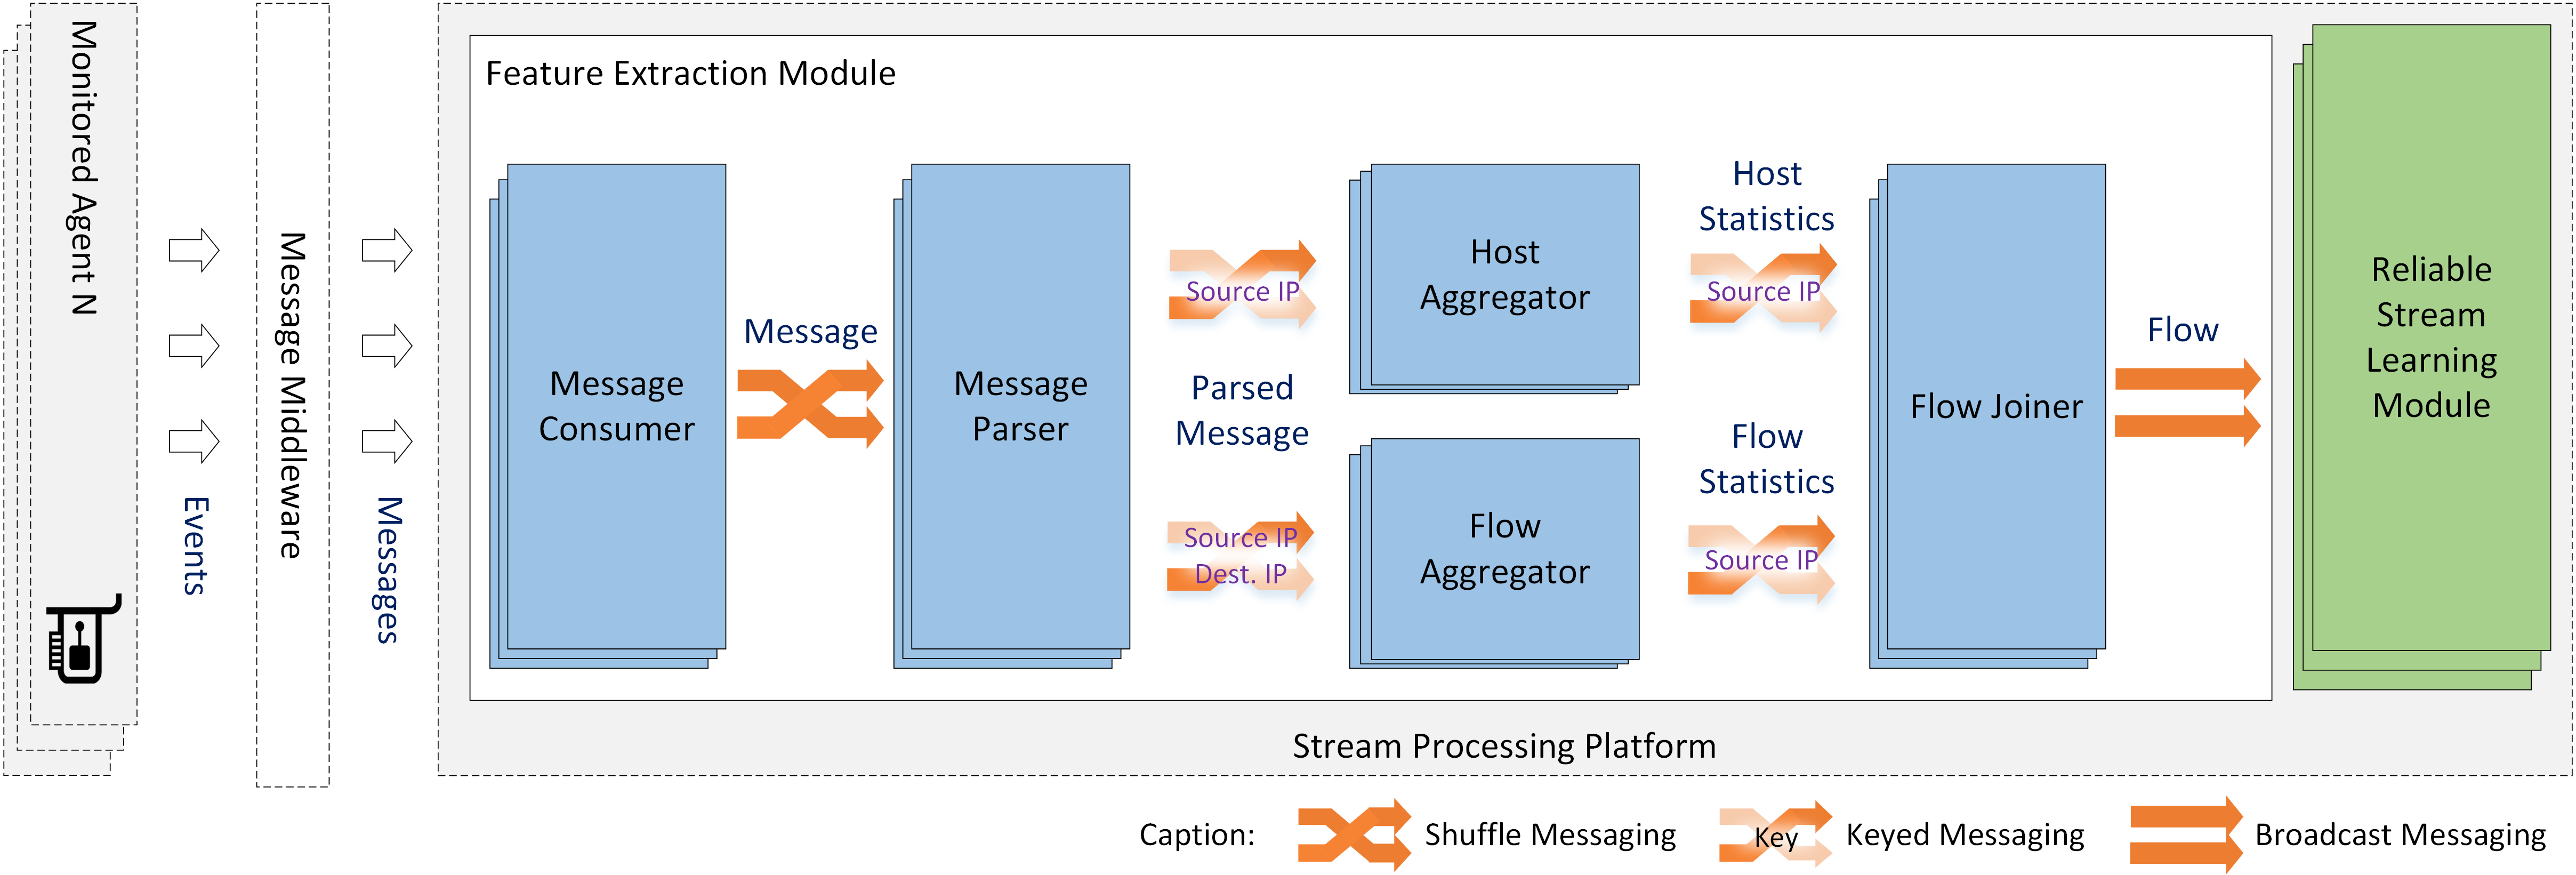
\includegraphics[width=\textwidth]{figuras/bigflow-fig2-feature_extraction_module.png}
% \caption{Módulo de extração de atributos da ferramenta BigFlow \cite{Viegas2019}.}
% \label{fig:bigflow-pcap}
% \end{figure}

% \begin{figure}[!ht]
% \centering
% 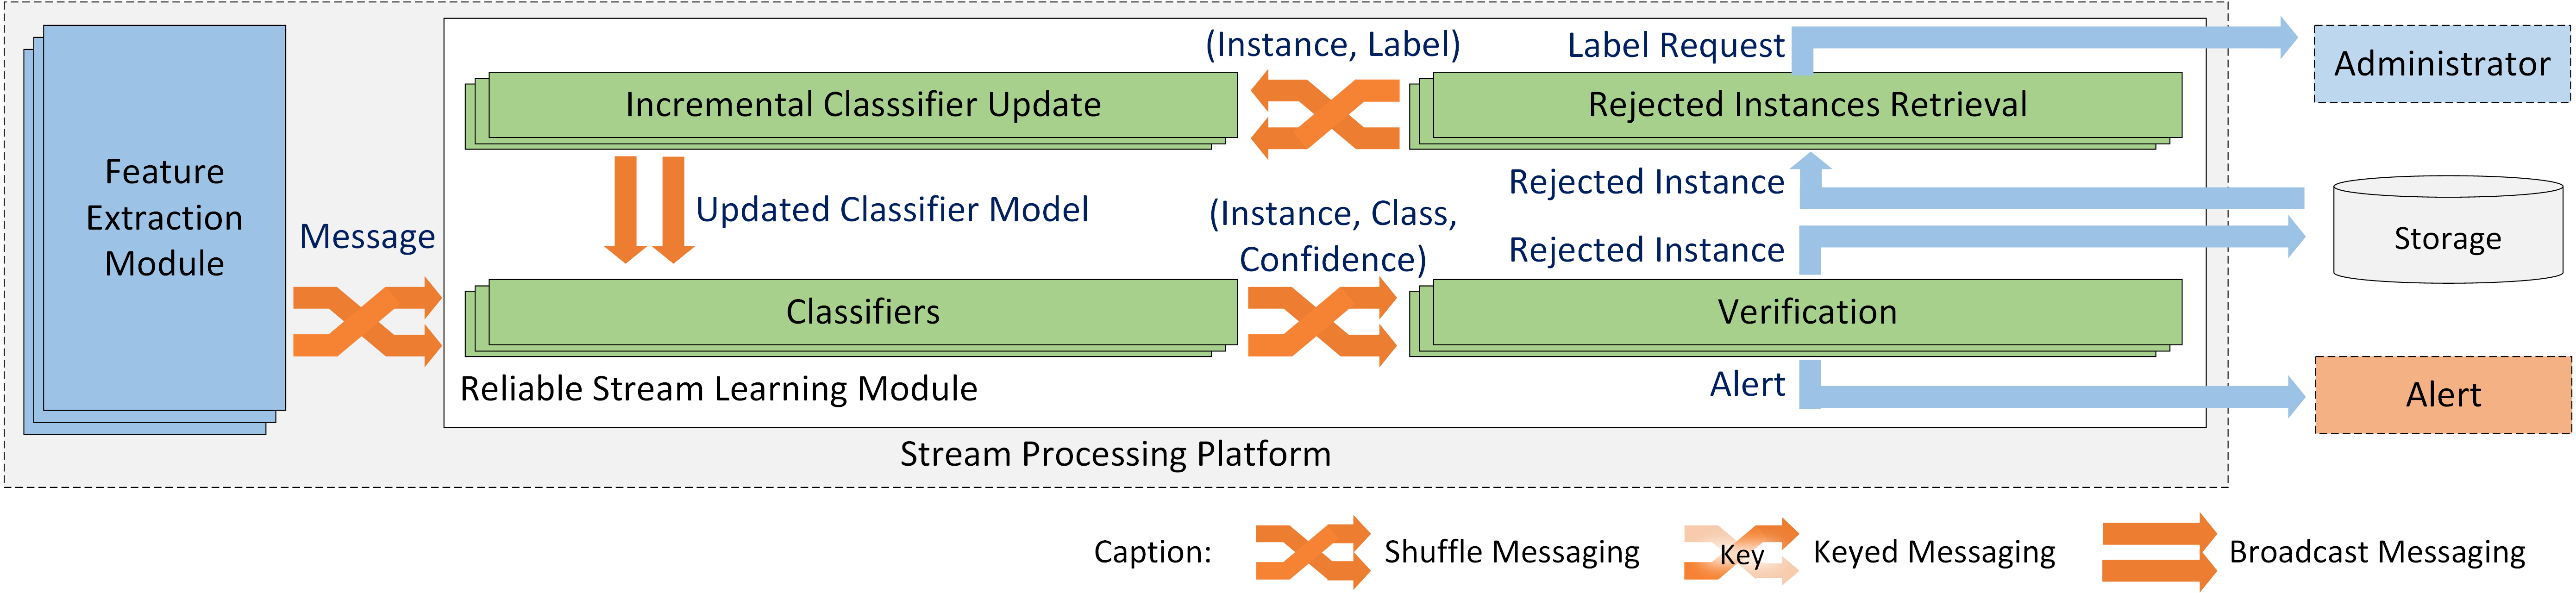
\includegraphics[width=\textwidth]{figuras/bigflow-fig4-reliable_learning_module.png}
% \caption{Módulo de aprendizado confiável da ferramenta BigFlow \cite{Viegas2019}.}
% \label{fig:bigflow-ml}
% \end{figure}

% BigFlow destaca em sua secção 2 (backgroud) o processamento de streams [18, 19],
% a preferencia de NIDS por anomalia em contraste aos NIDS por assinatura [30, 31, 32],
% a variabilidade e evolução dos padrões de tráfego em redes de propósito geral [9, 11, 20],
% a necessidade de atualização regular do modelo classificador [8, 9, 10, 20] e
% o tratamento de eventos onde a confiança resultante da classificação é baixa [9, 12, 13].

% [22] MAWI Working Group Traffic Archive, http://mawi.wide.ad.jp/mawi/samplepoint-F/.
% [24] H. He, E.A. Garcia, Learning from imbalanced data, IEEE Trans. Knowl. Data Eng.
% 21 (2009) 1263–1284. doi:10.1109/TKDE.2008.239.

\citeonline{Viegas2019} destaca que conjuntos de dados adequados para \nids são
poucos devido ao conjunto de qualidades que eles devem atender, como
realismo, validade, etiquetamento, grande variabilidade e reprodutibilidade
(disponibilidade pública).

% \notaPA{de ou do NIDS (?)}
Para avaliar o desempenho da proposta como um \nids, o conjunto de dados
MAWIFlow é proposto por \citeonline{Viegas2019}.
Este conjunto de dados é derivado dos traços de pacotes no \emph{backbone} WIDE, ponto de amostras F
(\emph{Packet traces from WIDE backbone, samplepoint-F}), composto por
seções diárias de captura de pacotes de 15 minutos de um link de $1\;
\mathrm{Gbps}$ entre Japão e EUA, com início em 2006 continuamente até hoje,
anonimizados e etiquetados por MAWILab \cite{mawiSamplepointF,Fontugne2010}.
Desse conjunto de dados original, o conjunto de dados MAWIFlow utiliza apenas os eventos de 2016,
dos quais $158$ atributos são extraídos resultando em $7.9\;\mathrm{TB}$ de captura de pacotes.
Por fim, os dados são estratificados para redução de seu tamanho a um
% centésimo, \hlhl{mantendo} as proporções de etiquetas (Ataque e Normal), \hlhl{facilitando} o
centésimo, mantendo as proporções de etiquetas (Ataque e Normal), facilitando o
compartilhamento e avaliação de NIDS, além de atender às qualidades anteriormente
mencionadas.

% classifiers that are usually employed for intrusion detection: decision tree
% (DT) [42], random forest (RF) [43], gradient boosting (GB) [44], and an ensemble
% [45] classifier composed from DT, RF, and GB that decides based on majority
% voting across each classifier’s decisions.

Com o conjunto de dados MAWIFlow reduzido a 62 atributos, foram avaliados quatro
classificadores da literatura em dois modos de operação.
% quanto aoseus dados de treinamento (ambos contendo uma semana de captura).
O primeiro modo de operação usa somente a primeira semana do ano como conjunto
de treinamento e as demais como conjunto teste.
O segundo modo usa o conjunto da semana anterior como treinamento e o
conjunto da semana seguinte como teste.
Comparando os resultados entre os modos de operação, os autores demonstram que a qualidade da
classificação reduz com o tempo quando não há atualização frequente do modelo
classificador.

Com base na avaliação dos classificadores da literatura, para a ferramenta
BigFlow é proposta a utilização de 4 algoritmos de classificação com capacidade
de atualização, sendo todos variações de árvore de decisão
\emph{Hoeffding} \cite{Viegas2019,Domingos2000}.
A avaliação da ferramenta foi executada de maneira semelhante à avaliação
dos algoritmos da literatura, onde o conjunto de dados da primeira semana foi
usado para treinamento e o conjunto de dados do restante do ano como conjunto
de teste. Em todos os casos a métrica observada foi a acurácia.
Além do conjunto de treinamento, o modelo é atualizado semanalmente com base nas
instâncias rejeitadas pelo submódulo de verificação. 
% , como ilustrado na \reffig{bigflow-ml}.

% four stream learning classifiers were evaluated:
% Hoeffding Tree [51], OzaBoosting [54], Leveraging Bag [55],
% and an Ensemble of the prior three classifiers that performs
% majority voting on the individual outcomes.

Quanto à distribuição do processamento,
%  ilustrada na \reffig{bigflow-arch},
a ferramenta BigFlow faz uso das plataformas \flink e \kafka.
Em especial, destaca-se o uso do serviço gerenciador de trabalhos (\emph{Job
Manager}) e as múltiplas instâncias do serviço gerenciador de tarefas
(\emph{Task Manager}).

% \begin{figure}[ht]
%   \centering
%   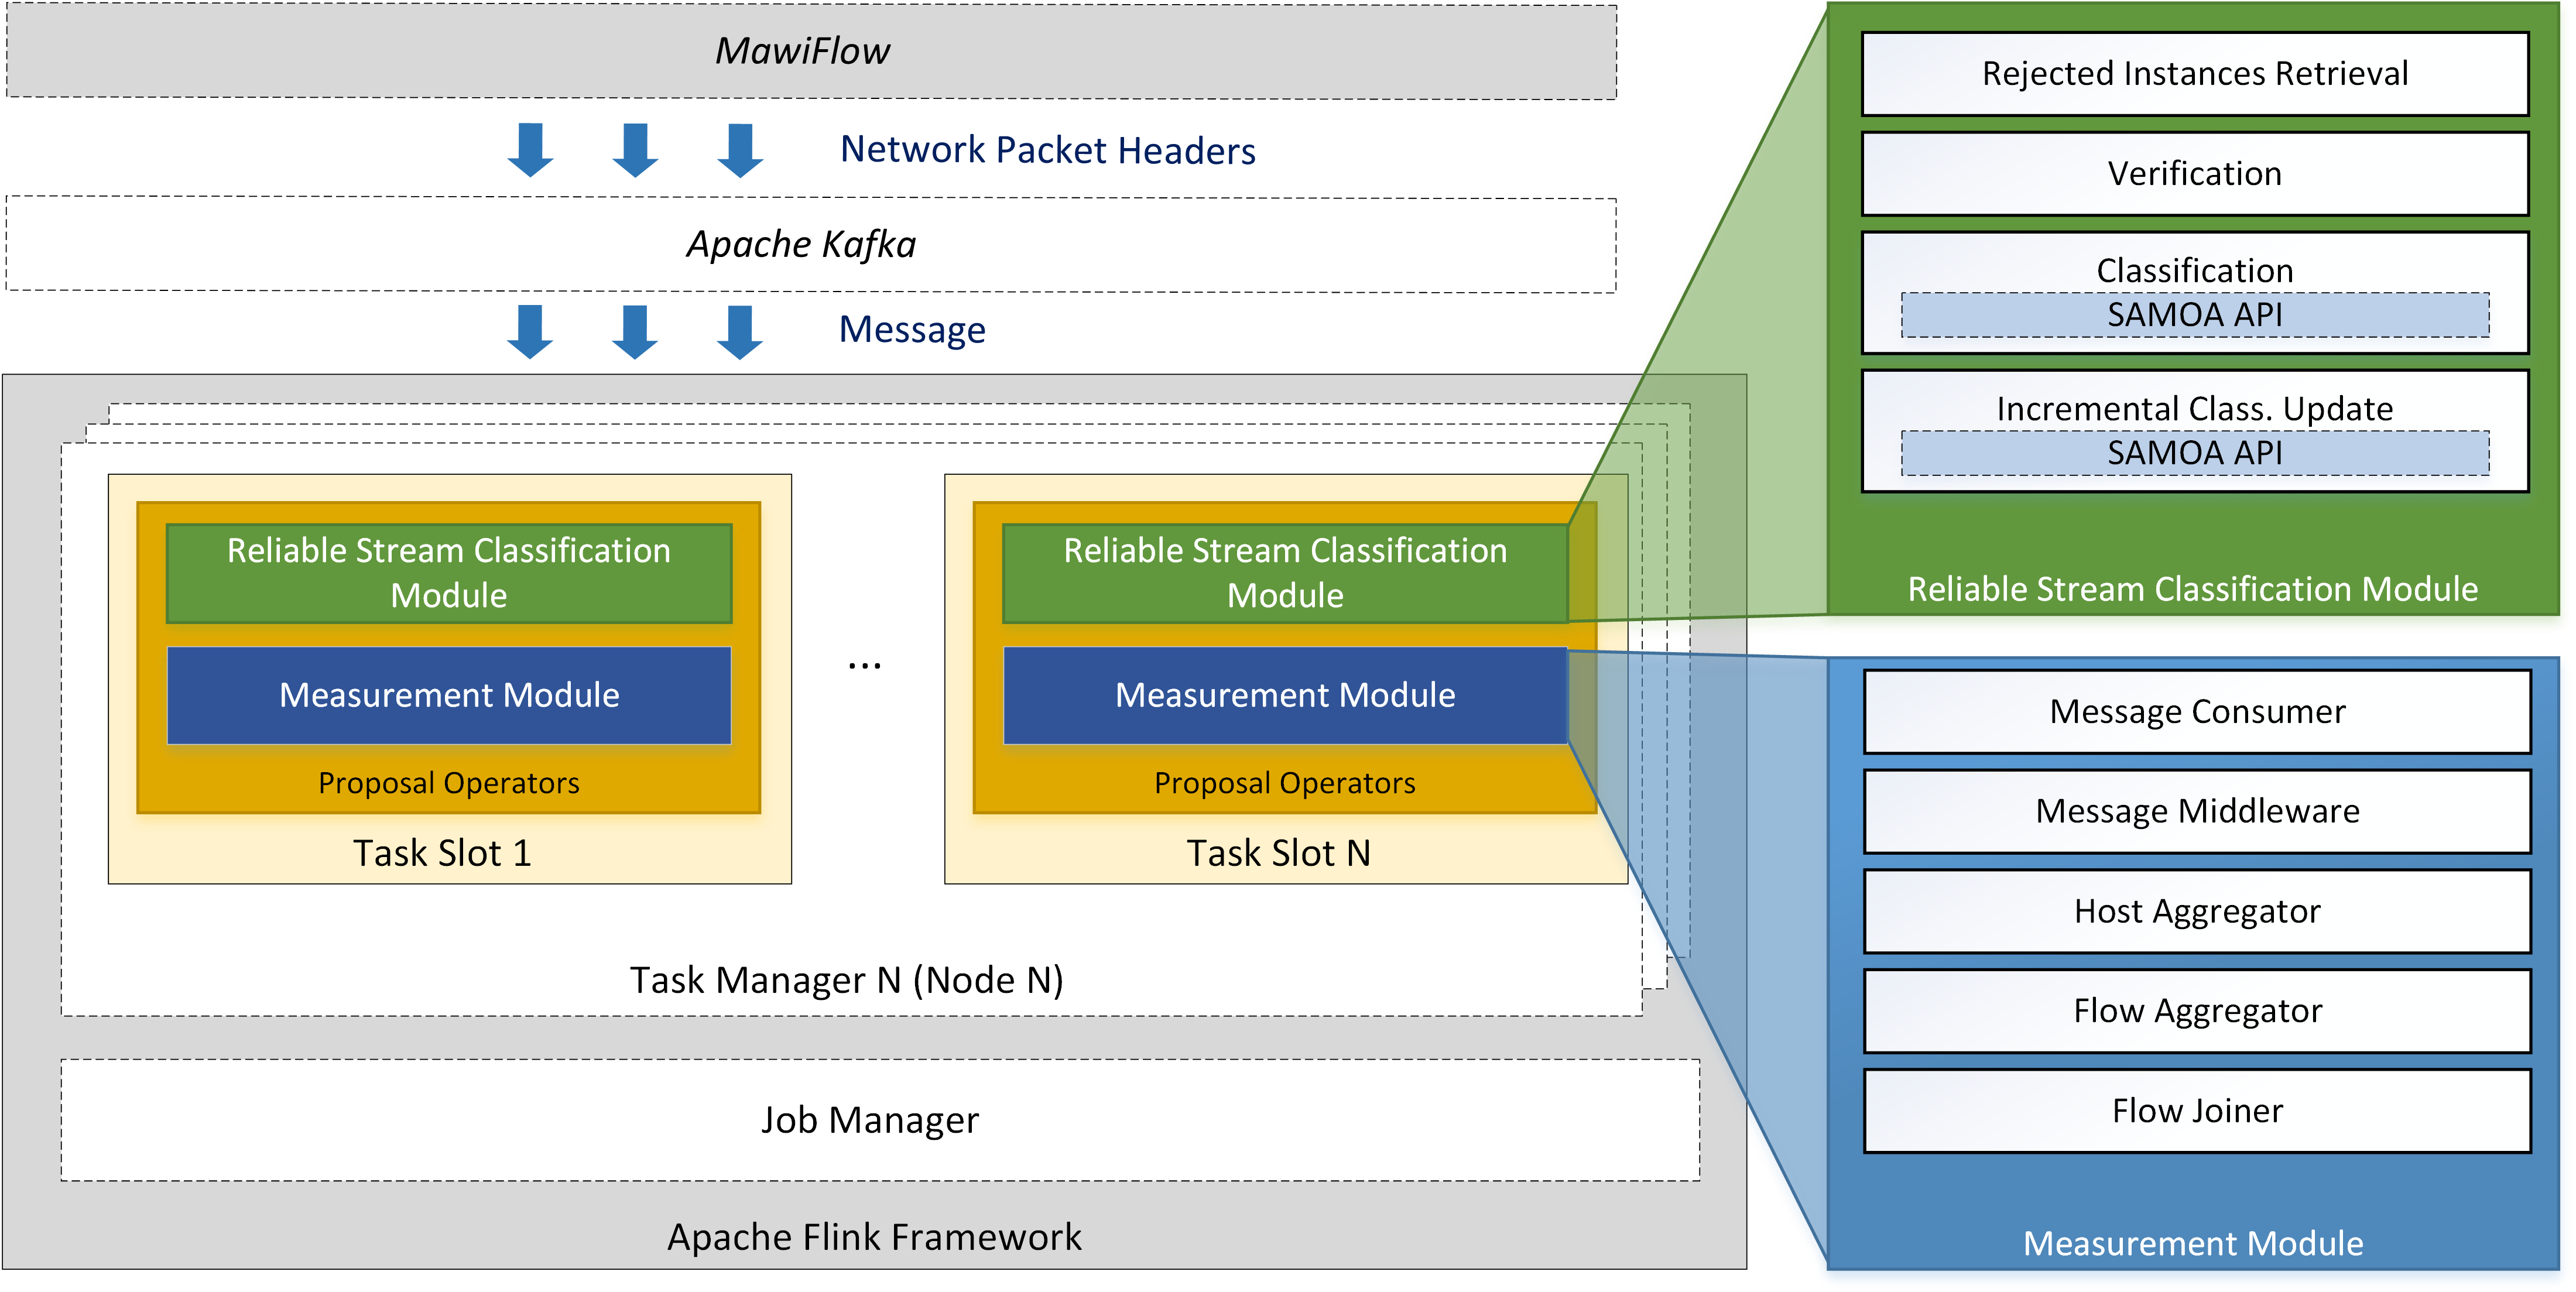
\includegraphics[width=\textwidth]{figuras/bigflow-fig5-bigflow_arch.png}
%   \caption{Visão geral da arquitetura e distribuição da ferramenta BigFlow \cite{Viegas2019}.}
%   \label{fig:bigflow-arch}
% \end{figure}

Em conclusão, a ferramenta BigFlow demonstra capacidade de classificação e
detecção de anomalias em fluxos de dados de alta velocidade no contexto de
detecção de intrusão.
No entanto a atualização semanal e a dependência da avaliação de um especialista
não são ideais para detecção de ameaças e respectiva ação sobre a descoberta de
novos padrões.

% Outras propostas tratam do caso de grandes volumes e velocidades, como ́e o caso
% de Viegas et al. (2019) que apresenta oBigFlow no intuito de detectar intrusão
% em redes10 GigabitEthernet, que ́e um volume considerável atualmente 
% impossível de ser processado em um ́único núcleo de processador (single-threaded).
% Essa implementação ́e feita sobre uma plataforma distribuída processadora
% de fluxos (Apache Flink) executada em um cluster com at ́e 10 n os de trabalho,
% cada um com 4 núcleos de processamento totalizando 40 núcleos para atingir
% taxas de até 10,72Gb ps.

\section{Ferramenta CATRACA}

O trabalho de \citeonline{Lopez2018} aborda a detecção de ameaças a redes de
computadores em tempo real e, para atingir esse objetivo, propôs a ferramenta
CATRACA\footnote{
    A ferramenta e sua documentação estão disponíveis em
    \url{http://gta.ufrj.br/catraca}
    e \url{https://github.com/tinchoa/catraca}.
}.
A ferramenta CATRACA é composta de três camadas: captura, processamento e
visualização.
%  ilustradas na Figura \ref{fig:catraca}.

% \begin{figure}[ht]
% \centering
% 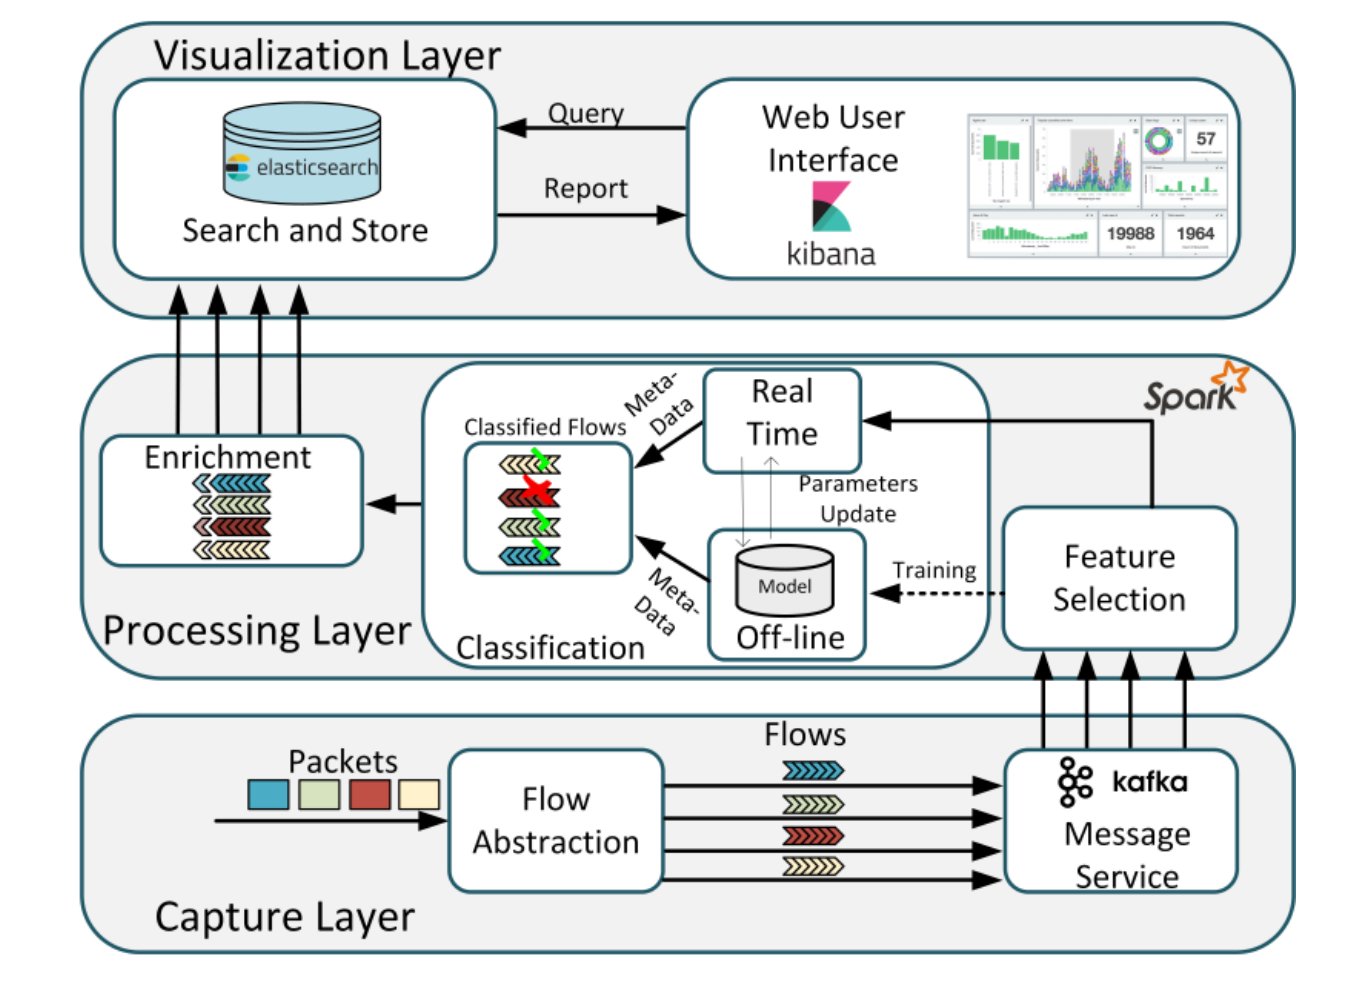
\includegraphics[width=0.8\textwidth]{figuras/catraca-arch.png}
% \caption{Arquitetura em camadas da ferramenta CATRACA \cite{Lopez2018}.}
% \label{fig:catraca}
% \end{figure}

% \nota{deu pra entender,mas coloca ou vírgula, ou divide as frases: baseada na
% biblioteca flowbag. Essa biblioteca é embalada ou a funcao em python esta
% embalada em um funcao virtual de rede?}

Na camada de captura, pacotes são capturados da rede e 
são gerados descritores de fluxos
por uma aplicação \emph{Python} utilizando a biblioteca \emph{flowtbag}\footnote{
    Disponível em \url{https://github.com/danielarndt/flowtbag} e
    \url{https://dan.arndt.ca/projects/netmate-flowcalc/}.
}.
Esses descritores de fluxo são enviados para um tópico de um sistema de fila de mensagens
(\emph{Apache Kafka}) hospedado em nuvem.
Essa aplicação \emph{Python} é distribuída como uma função virtual de rede
(\emph{Network Function Virtualization}) executada em dispositivos virtuais de rede.
% hospedados em névoa

% estabelecendo um ambiente de computação em névoa.
A camada de processamento consome o tópico de mensagens que contém os descritores de fluxos
da camada de captura e extrai características dos descritores de fluxos, detecta e classifica ameaças,
enriquece o resultado (com localização geográfica por exemplo) e envia para a
próxima camada na arquitetura por meio de um banco de dados.
A última camada da ferramenta fornece uma interface gráfica que apresentada a
visualização dos descritores de fluxos processados bem como os conhecimentos extraídos e
armazenados no banco de dados.
Ambas as camadas de processamento e visualização são executadas em ambiente de
computação em nuvem.

Para o desenvolvimento da ferramenta CATRACA, \citeonline{Lopez2018} avaliou e
comparou as plataformas de processamento de fluxo de dados em tempo real
disponíveis (\emph{Apache Storm}, \emph{Apache Flink}, \emph{Apache Spark Streaming}).
A avaliação extraiu a velocidade máxima, em mensagens por minuto,
de cada plataforma, variando a configuração de paralelismo
em dois programas.
Ambos consumiam dados de um tópico de um sistema de fila
de mensagens (\emph{Apache Kafka}) e produziam para outro tópico.
O primeiro programa consiste de um detector de ameaças composto por
uma rede neural classificadora escrito em \emph{Java}, que foi testado
com o conjunto de dados sintético UFRJ/GTA \cite{Lopez2018}.
O segundo programa conta quantas repetições de uma palavra existem em um
fluxo de dados, exemplo muito comum em tutoriais de plataformas desse gênero,
e é avaliado com um conjunto de \emph{Tweets}.

% Nesta avaliação, \emph{Apache Storm} foi capaz de processar até 15 milhões de
% mensagens por minuto
% 
% We described and compared the three-major open source distributed stream
% processing systems: Apache Storm, Apache Flink, and Apache Spark Streaming. We
% performed throughput analysis, allocating more processing cores to achieve
% higher processing rates, Apache Storm was able to process up to 15 million
% samples per minute. Moreover, we performed fault tolerance test to compare these
% three most popular open-source Distribute Stream Processors (DSP). In this case,
% we showed that Spark streaming, using micro-batch processing model, can recover
% the failure without losing any messages. Spark Streaming stores the full
% processing state of the micro-batches and distributes the interrupted processing
% homogeneously among other worker nodes.

% A comparação envolveu:
% \begin{enumerate}
%     \item Apache Storm versão 0.9.4 de 2015-03-18 (atualmente na versão 2.1.0,
%     publicada em 2019-10-25);
%     \item Apache Flink versão 0.10.2 de 2016-02-03 (atualmente na versão 1.10.0,
%     publicada em 2020-02-11);
%     \item Apache Spark Streams versão 1.6.1 de 2016-02-27 (atualmente na versão
%     2.4.5, publicada em 2020-02-02);
% \end{enumerate}
% Além das plataformas comparadas é importante mencionar a presença em todos os
% testes do Apache Kafka na versão 0.8.2.1 de 2015-02-26 (atualmente na versão
% 2.4.0 de 2019-12-13).
% A estratégia de avaliação continha um 
% Os resultados apresentados por essa avaliação mostraram que Apache Storm 

Para o modelo de classificação, a ferramenta CATRACA utiliza o método árvore de
decisão, escolhido pelo rápido treinamento e pela alta precisão e acurácia\footnote{
    A precisão e a acurácia do método árvore de decisão podem estar associadas
    à independência entre as características (\emph{features}) de cada exemplo,
    típico de conjuntos derivados de pacotes de rede.
}.
O modelo é criado na fase \emph{Offline} e utilizado na classificação binária
(normal e ameaça) da fase \emph{Online}, sendo recalculado quando uma ameaça
é encontrada.

% test\\
% $214200$\\
% $214\,200$\\
% $214\, 200$\\
% $214\;200$\\
% $214\; 200$\\
% $214200$\\

Pra avaliação da ferramenta CATRACA dois conjuntos de dados são utilizados.
O primeiro conjunto, UFRJ/GTA, é sintético e foi criado por uma simulação de
rede de computadores, contendo $214\;200$ fluxos de rede e totalizando $95\;
\mathrm{GB}$ de pacotes capturados, este conjunto de dados
é composto de 24 atributos e 16 classes.
O outro conjunto, referido como NetOp, foi coletado de um operador de rede que
atendia 373 residências na cidade do Rio de Janeiro em 2017.
O conjunto NetOp é formado por 5 TB de pacotes capturados e etiquetados por um
detector de intrusão comercial.

Também para a avaliação da ferramenta CATRACA, foram utilizadas as métricas de qualidade
de classificação acurácia, precisão, sensibilidade e F1M, com intervalo de
confiança de $95\%$.
As métricas de qualidade, dependendo do tamanho do conjunto, foram extraídas por
métodos de avaliação amplamente utilizados para avaliar modelos de aprendizado
de máquina (\emph{machine learning}) como validação cruzada com proporção
$70\%$ do conjunto base para treinamento e $30\%$ para teste.
Para as métricas de escalabilidade foram utilizadas a latência e fator de aceleração
(\emph{speedup}).

Em conclusão, a ferramenta CATRACA apresenta uma arquitetura dividida em camadas
alocadas em ambientes de névoa e nuvem.
Essa ferramenta foi avaliada com métricas de qualidade, métricas de
escalabilidade e dois conjuntos de dados relevantes.
No entanto, o algoritmo de detecção de anomalias desenvolvido para a ferramenta
consiste de um modelo de classificação pelo método árvore de decisão e
a atualização do modelo durante a fase \emph{Online} depende de todos os exemplos do
último intervalo de atualização.
% Esse tipo de algoritmo de detecção de anomalias 
% \notahl{por que não?}
% \hlhl{não é capaz de lidar}
% \hlhl{adequadamente com as características de fluxos contínuos} de dados, como os
% descritos na \refsec{nd} (\drift, \evolution, limitado a ler o conjunto somente
% uma vez), que são atendidos por algoritmos de detecção de novidade.

% A monitoring and threat detection system using stream processing as a virtual 
% function for Big Data

% A detecção tardia de ameaças de segurança causa um significante aumento no
% risco de danos irreparáveis, impossibilitando qualquer tentativa de defesa.
% Como consequência, a detecção rápida de ameaças em tempo real é essencial
% para a ad- ministração de segurança. Além disso, A tecnologia de
% virtualização de funções de rede (Network Function Virtualization - NFV)
% oferece novas oportunidades para soluções de segurança eficazes e de baixo
% custo. Propomos um sistema de detecção de ameaças rápido e eficiente,
% baseado em algoritmos de processamento de fluxo e de aprendizado de máquina. As
% principais contribuições deste trabalho são: 
% i) um novo sistema de monitoramento e detecção de ameaças baseado no processamento de fluxo; 
% ii) dois conjuntos de dados, o primeiro é um conjunto de dados sintético de
% segurança contendo tráfego suspeito e malicioso, e o segundo corresponde a uma
% semana de tráfego real de um operador de telecomunicações no Rio de Janeiro,
% Brasil; 
% iii) um algoritmo de pré-processamento de dados composto por um algoritmo
% de normalização e um algoritmo para seleção rápida de
% características com base na correlação entre variáveis;
% iv) uma função de
% rede virtualizada em uma plataforma de código aberto para fornecer um serviço
% de detecção de ameaças em tempo real;
% v) posicionamento quase perfeito de
% sensores através de uma heurística proposta para posicionamento estratégico
% de sensores na infraestrutura de rede, com um número mínimo de sensores; e,
% finalmente, 
% vi) um algoritmo guloso que aloca sob demanda uma sequência de 
% funções de rede virtual.

\section{Arquitetura \arch}\label{sec:cassales}

A arquitetura \arch, proposta por \citeonline{Cassales2019}, tem por objetivo
monitorar uma rede local com dispositivos \iot e detectar tentativas de intrusão
e alguma subversão do comportamento das transmissões destes dispositivos.
O principal destaque da arquitetura é a distribuição de tarefas do sistema de
detecção de intrusão entre nós de névoa e nós em nuvem pública.
O objetivo dessa distribuição é a redução de latência, que torna inviável a
hospedagem de um sistema detector de intrusão somente em ambiente de nuvem, e
também possibilitar a análise de grandes volumes de dados por algoritmos de
maior complexidade, que são de custo computacional proibitivo para nós de borda.

A arquitetura proposta é avaliada com três algoritmos de detecção de novidade:
ECSMiner \cite{Masud2010ECSMiner}, AnyNovel \cite{Abdallah2016anynovel} e \minas
\cite{Faria2016minas}.
A avaliação foi feita com o conjunto de dados \emph{Kyoto 2006+}, composto de
dados coletados de 348 \emph{Honeypots} 
(máquinas isoladas, equipadas com diversos
softwares com vulnerabilidades conhecidas e expostas à Internet, com propósito de
atrair ataques) de 2006 até dezembro 2015.
Esse conjunto de dados tem as características desejáveis de um conjunto para detecção de
novidades como: realismo, validade, etiquetas previamente definidas, alta
variabilidade, reprodutibilidade e disponibilidade pública.
O conjunto de dados \emph{Kyoto 2006+} contém 24 atributos, 3 etiquetas atribuídas por
detectores de intrusão comerciais e uma etiqueta
distinguindo o tráfego entre normal, ataque conhecido e ataque desconhecido.

A avaliação da arquitetura foi realizada utilizando as métricas de qualidade
\emph{Fnew}, \emph{Mnew} e \emph{erro}.
A métrica \emph{Fnew} (ou Falso Positivo) é a fração dos exemplos de uma classe normal
classificados com etiqueta novidade ou etiqueta extensão.
A métrica \emph{Mnew} (ou Falso Negativo) é a fração dos exemplos de uma classe novidade
classificados com etiqueta normal.
A métrica \emph{erro} é a soma dos valores falso positivo e falso negativo dividida
pelo número de exemplos classificados.
Além das métricas de qualidade de classificação tradicionais, também foi medida
a quantidade de requisições de classificação por especialista.

Outra avaliação dos algoritmos foi a extração de métricas de uso de recursos
computacionais e tempo total de processamento em dispositivos limitados.
Essa avaliação envolveu dois computadores.
Para tanto, um computador pessoal com recursos
convencionais produzia exemplos e adicionava como mensagens em um tópico no
sistema de fila de mensagens \kafka; já o outro computador, com recursos
limitados, consumia as mensagens do tópico e classificava os exemplos.

Ambas as avaliações demonstraram o equilíbrio entre qualidade de classificação e
velocidade ou uso de recursos.
O algoritmo ECSMiner mostrou melhor qualidade de classificação, porém com
velocidade inferior e maior consumo de recursos comparado aos outros algoritmos.
Já o algoritmo \minas, apesar de maiores valores na métrica \emph{erro}, mostrou-se
adequado para dispositivos limitados com baixo consumo de recursos
computacionais e manteve a métrica \emph{Fnew} constante e baixa.
O algoritmo AnyNovel não apresentou consistência nos resultados e o consumo
de recursos computacionais (memória) foi elevado.

% MINAS technique presented high error rates. However, the
% small and constant \emph{Fnew} coupled with the smallest execution
% time and memory consumption, indicates MINAS is suitable
% for IoT scenarios.

A proposta de distribuição das tarefas em serviços abre oportunidades para a
discussão de diferentes métodos de distribuição dessas tarefas em diferentes
ambientes computacionais.
Contudo, o algoritmo \minas que apresentou resultados promissores para este tipo de cenário ainda não foi implementado e avaliado com
paralelismo e distribuição que são necessários para tratar fluxos de dados com
grandes volumes de dados e velocidades.

% \nota{Também discutir a classificação dos fluxos por endpoint
% exarcerbando assim a distinção na fog com o efeito de particionamento dos dados.
% Ou seja, um nó só vê e classifica os próprios dados.}

% \section{Conjuntos de Dados e Referência de Desempenho para Detecção de Anomalia}

% The Numenta Anomaly Benchmark
% - Airline, approximately 116 million flight arrival and departure records
%   (cleaned and sorted) compiled by E. Ikonomovska. Reference: Data Expo 2009
%   Competition [1]. Access
% - Chess.com (online games) and Luxembourg (social survey) datasets compiled by
%   I. Zliobaite. Access
% - ECUE spam 2 datasets each consisting of more than 10,000 emails collected over
%   a period of approximately 2 years by an individual. Access from S.J.Delany
%   webpage
% - Elec2, electricity demand, 2 classes, 45,312 instances. Reference: M. Harries,
%   Splice-2 comparative evaluation: Electricity pricing, Technical report, The
%   University of South Wales, 1999. Access from J.Gama webpage. Comment on
%   applicability.
% - PAKDD'09 competition data represents the credit evaluation task. It is
%   collected over a five-year period. Unfortunately, the true labels are released
%   only for the first part of the data. Access
% - Sensor stream and Power supply stream datasets are available from X. Zhu's
%   Stream Data Mining Repository. Access
% - SMEAR is a benchmark data stream with a lot of missing values. Environment
%   observation data over 7 years. Predict cloudiness. Access
% - Text mining, a collection of text mining datasets with concept drift,
%   maintained by I. Katakis. Access
% - Gas Sensor Array Drift Dataset, a collection of 13,910 measurements from 16
%   chemical sensors utilized for drift compensation in a discrimination task of 6
%   gases at various levels of concentrations. Access

\section{Síntese dos trabalhos relacionados}\label{sec:conclusao-relacionados}

% \nota{coloca uma secao de SINTESE dos trabalhos relacionados ou sintese do capitulo}

Os trabalhos discutidos nesse Capítulo têm temas complementares em
áreas distintas.
A área de aprendizado de máquina, com o tema detecção de novidades em fluxos de
dados, preocupa-se em fornecer melhores previsões através de algoritmos
classificadores que atendam as características de cada problema.
A área de computação distribuída aborda os temas de processamento distribuído
de fluxos contínuos em ambientes de computação em nuvem e em névoa, fornecendo
métodos para processar grandes volume de dados com mínima latência.

Um sumário dos trabalhos abordados pode ser visto na Tabela \ref{tab:summary}.
% \notaPA{Falta a comparação com a sua proposta. Quais as diferenças? O que há de
% melhor/pior?}
% \nota{TODO: Fazer novo parágrafo de comparação}
Destaca-se a lacuna encontrada onde não há uma implementação de detector de
intrusos focada na execução em ambiente de névoa com recursos limitados.
Além disso, as propostas existentes que tratam grande volume de dados, como
BigFlow \cite{Viegas2019} e CATRACA \cite{Lopez2018}, não oferecem atualização
de modelo contínua sem interação com um especialista externo.
No entanto, o \emph{speedup} alcançado neste trabalho ficou abaixo do esperado,
onde, por exemplo, no trabalho de \citeonline{Lopez2018} foi obtido o
\emph{speedup} $4.65$ para $20$ processadores, enquanto este trabalho observou
$0.97$ para $12$ processadores.

\begin{table}[ht]
  \caption{Sumário dos trabalhos relacionados}
  \centering
  \begin{scriptsize}
  \begin{tabularx}{\linewidth}{X|X|X|X|X|X}
    \textbf{Trabalho} &
        \textbf{Plataforma} &
        \textbf{Técnica ou Algoritmo} &
        \textbf{Atualização de Modelo} &
        \textbf{Conjunto de dados} &
        \textbf{Métricas} \\
    \hline & & & & & \\
    Ferramenta BigFlow \cite{Viegas2019} &
        \python, \emph{flowtbag}, \kafka e \flink &
        \emph{Hoeffding Tree}, \emph{OzaBoosting}, \emph{Leveraging Bag} e comitê &
        Semanal semi-automática &
        \emph{MAWILab} &
        Acurácia (geral e por classe), Taxa de bytes \\
    \hline & & & & & \\
    Ferramenta CATRACA \cite{Lopez2018} &
        \emph{Virtual Network Function}, \kafka e \spark &
        PCA, SFS, e SVM-RFE &
        Contínua semi-automática &
        NSL-KDD, GTA/UFRJ e NetOp &
        Acurácia, precisão, sensibilidade e F1-score \\
    \hline & & & & & \\
    Arquitetura \arch \cite{Cassales2019} &
        Java, \kafka e \python &
        ECSMiner, AnyNovel e MINAS &
        Contínua Automática &
        \emph{Kyoto 2006+} &
        \emph{Fnew}, \emph{Mnew} e \emph{erro}
    % Murilo Naldi da UFSCAR & plataforma & técnica & conjunto de dados & métricas \\
    % Não encontrei uma plataforma do Naldi, encontrei algoritmos.
    % \hline
    % Latifur Khan & plataforma & técnica & conjunto de dados & métricas \\
    % \hline
    % CLAM & plataforma & técnica & conjunto de dados & métricas \\
    % \hline
    % trabalhos do Bifet e o framework baseado no MOA (samoa) & plataforma & técnica & conjunto de dados & métricas \\
    % \hline
  \end{tabularx}
  \label{tab:summary}
  \end{scriptsize}
\end{table}

% Apesar de já existirem propostas que estabelecem o estado da arte separadamente
% em cada um dos temas, \hlhl{falta ainda uma abordagem que estabeleça uma união} entre o
% estado da arte em \hlhl{algoritmos de detecção} de novidade e o estado da arte em
% \hlhl{processamento distribuído} de fluxos de dados, em especial para \hlhl{o ambiente de
% computação em névoa} focado em \hlhl{fluxos de dados} relacionados a \hlhl{dispositivos \iot.}
